\documentclass{etit-workshop-protokoll}
\usepackage[outdir=./]{epstopdf}
\usepackage{graphicx}
\usepackage{multirow}
\usepackage{adjustbox}
\usepackage{xcolor}
\usepackage{amsmath}
\usepackage{framed}
\usepackage{wrapfig}
\usepackage{lscape}
\usepackage{rotating}

\colorlet{shadecolor}{gray!0}

%\kursnummer{0}
%\kurstitel{Leitfaden und Vorlage zur Ausarbeitung}

%\kursnummer{1}
%\kurstitel{Messwerterfassung und regenerative Energieerzeugung}

\kursnummer{2}
\kurstitel{Analoge Filter und Schaltungsanalyse}

%\kursnummer{3}
%\kurstitel{Sensorik}

%\kursnummer{4}
%\kurstitel{Digitale Signalverarbeitung}


\gruppennummer{14}

\teilnehmer{Lucas Antonie}{Romier}{2214444}{ukhie}{lucas.romier@gmail.com}
\teilnehmer{Aleksandra Marta}{Wrzeszcz}{2239492}{ubsyj}{a.wrzeszcz98@o2.pl}
\teilnehmer{Timo Johannes}{Weber}{2253834}{uhoiz}{timo_weber@online.de}

\newcommand{\gleichung}[2]{
\begin{framed}
\begin{center}
\begin{equation}
#1
\label{#2}
\end{equation}
\end{center}
\end{framed}
}

\begin{document}

\maketitle

\pagestyle{empty}% % leere Kopfzeile
\clearpage % neue Seite beginnen
\pagestyle{scrheadings} % Kopfzeilen zuruecksetzen

\tableofcontents
\listoffigures
\clearpage
\listoftables

\clearpage % neue Seite beginnen
\section{Vorbereitung}

\noindent{\large Arbeitsaufteilung:\par}
\begin{table}[htb]
\centering
\caption{Arbeitsaufteilung in der Gruppe}
\label{Arbeitsaufteilung}
\begin{tabular}{c|ccc}
\toprule
Aufgabe & Lucas & Aleksandra & Timo\\
\midrule
Motivation &  & x & \\
Literaturrecherche &  &  & x\\
1.2 Filterschaltungen & x & x & x\\
1.3 Addierschaltung & x & x & x\\
Dokumentation & x & x & x\\
Diskussionen & x & x & x\\
Bericht \& Spice & x &  & \\
\bottomrule
\end{tabular}
\end{table}

\noindent{\large Genutzte Materialien:\par}
\begin{table}[htb]
\centering
\caption{Genutzte Materialien}
\label{Arbeitsaufteilung}
\begin{tabular}{c|c|c}
\toprule
Bauteiltyp & Beschreibung & Wert\\
\midrule
Digital-Analog-Wandler & MCP4922, 1x & \\
\hline
Operationsverstärker & MCP6002, 4x & \\
\hline
Kondensatoren & 
\vtop{
\hbox{\strut Keramik- und}
\hbox{\strut Elektrolytkondensatoren,}
\hbox{\strut bis 100 nF: 10\% Toleranz,}
\hbox{\strut ab 470 nF: 20\% Toleranz,}
\hbox{\strut 4x oder 2x}
}
& 
\vtop{
\hbox{\strut diverse:}
\hbox{\strut ~~~~10 nF, 22 nF, 33 nF}
\hbox{\strut ~~~~47 nF, 68 nF, 100 nF}
\hbox{\strut ~~~~470 nF, 10 $\mu$F, 100 $\mu$F}
}
\\
\hline
Widerstände &
\vtop{
\hbox{\strut Kohleschichtwiderstände,}
\hbox{\strut 1/4 W,}
\hbox{\strut 5\% Toleranz,}
\hbox{\strut jeweils 10x}
}
& 
\vtop{
\hbox{\strut E6-Reihe:}
\hbox{\strut ~~~~100$\Omega$, 220$\Omega$, 470$\Omega$}
\hbox{\strut ~~~~1 k$\Omega$, 1,5 k$\Omega$, 2,2 k$\Omega$}
\hbox{\strut ~~~~3,3 k$\Omega$, 4,7 k$\Omega$, 6,8 k$\Omega$}
\hbox{\strut ~~~~10 k$\Omega$, 15 k$\Omega$, 22 k$\Omega$}
\hbox{\strut ~~~~33 k$\Omega$, 47 k$\Omega$, 68 k$\Omega$}
\hbox{\strut ~~~~100 k$\Omega$, 220 k$\Omega$, 1 M$\Omega$}
}
\\
\hline
Potentiometer & Potentiometer, 2x & 0...100 k$\Omega$\\
\bottomrule
\end{tabular}
\end{table}

\clearpage
\section{Einleitung}

\subsection{Motivation}
Die vorliegende Dokumentation gibt einen Überblick über unsere Arbeit im Rahmen des Workshops ”Analoge Filter und Schaltungsanalyse - Entwicklung eines 2-Band-Equalizers”.
\\
\\
Mittels der in Tabelle 1 dargestellten Materialien wurde eine komplexe Analyse und Aufbau eines Filters durchgeführt. 
\\
\\
Zunächst wird ein allgemeiner Überblick der Funktion von Filtern verschiedener Ordnung gegeben. Im Folgenden wird Schritt für Schritt die Theorie mit entsprechenden Kommentaren praktisch umgesetzt, zusammen mit Bildern der Schaltungen und Diagrammen, die
deutlich die Funktionalität der Filter zeigen. Abschließend wird das Resultat unserer Arbeit in einem von uns durchgeführten Praxistest kurz zusammengefasst.

\subsection{Literaturrecherche}
Grundlagen
In der Elektrotechnik bezeichnet ein Filter eine Schaltung, die sich bei verschiedenen Eingangsfrequenzen unterschiedlich verhält. Genauer bedeutet dies, dass schaltungsabhängig bestimmte Frequenzbereiche entweder verstärkt, gedämpft oder nicht beeinflusst werden. Zudem wird die Phasenverschiebung zwischen Ein- und Ausgangssignalen beeinflusst. Aufgrund dieser Eigenschaften finden Filterschaltungen Einsatz in unterschiedlichsten Anwendungen. Die gängigsten Filterarten sind der Hochpass, der tiefe Frequenzen dämpft und, wie der Name andeutet, hohe Frequenzen passieren lässt, der Tiefpass, der das Gegenstück zum Hochpass bildet, ebenso wie Bandpass und Bandsperre. Diese dämpfen nur Frequenzen innerhalb oder außerhalb eines bestimmten Frequenzbandes.
Bandpassfilter werden zum Beispiel in der Telekommunikationstechnik, für den Rundfunk und in der Musikproduktion eingesetzt. Tiefpassfilter mit hoher Flankensteilheit werden zum Beispiel für die Datenverarbeitung verwendet, um Störsignale auszufiltern. Einen Spezialfall bilden die Allpassfilter, die keine Frequenzen dämpfen, sondern nur zur Phasenverschiebung verwendet werden.
Die Klassifizierung von Filtern erfolgt in der Regel über ihre Funktion, Ordnung, Bauteilzusammensetzung und ihre Bauteilwerte. Passive Filter enthalten nur passive Bauelemente wie Kondensatoren, Widerstände und Spulen. Spulen und Kondensatoren fungieren hierbei als frequenzabhängige Widerstände und bestimmen die Kennwerte des jeweiligen Filters. Aktive Filter hingegen enthalten mindestens ein aktives Bauelement, wie Transistoren oder Operationsverstärker. Aktive Filter benötigen demnach eine externe Spannungsversorgung, um das aktive Element einsatzfähig zu machen und den Filter betreiben zu können.
Eine Kenngröße eines Filters ist seine Ordnung. Der Wert der Ordnung eines Filters wird über dessen Steigung im Dämpfungsbereich des Bode-Diagramms ermittelt. Ein Filter mit Flankensteigung von 20dB/Dek hat eine Ordnung von 1. Pro zusätzlichen 20dB/Dek steigt die Filterordnung um 1. Demnach besitzt ein Filter mit einer Flankensteigung von 40dB/Dek eine Ordnung von 2. 
Die Grenzfrequenz ist eine weitere wichtige Kenngröße von Filtern. Sie definiert den Übergang zwischen Durchlass- und Sperrbereich eines Filters und stellt die Frequenz dar, bei der das Signal des Filters um 3dB bzw. den Faktor $\sqrt{2}$ gedämpft wird.
Die Knickfrequenz hingegen beschreibt die Frequenz, die sich an dem Schnittpunkt der Tangenten des Durchlass- und Sperrbereichs ermitteln lässt. \cite{tkotz} \cite{kendall} \cite{tietze} 
\\
\\
Der charakteristische Amplituden- und Phasengang eines Filters wird in einem Bode-Diagramm dargestellt. Hierbei wird die Verstärkung oder Dämpfung der Amplitude des Eingangssignals und dessen Phasenverschiebung über einer logarithmischen Frequenzskala aufgetragen. \cite{tkotz} \cite{tietze} 
\\
\\
Zur Beschreibung eines Filters wird guter Letzt noch der Qualitätsfaktor Q benötigt. Dieser beschreibt die Eigenschwingung bei Tief- und Hochpassfiltern. Für den Fall, dass der Wert Q gegen $\infty$ geht wird der Filter zum Oszillator, wodurch der Filter seine Funktion nicht mehr erfüllt und benachbarte Schaltungsteile beschädigen könnte. Für Q zwischen 1/2 und 0 filtert der Filter nicht mehr alle ungewünschten Frequenzen heraus, sondern lässt teilweise ungewünschte Frequenzen ungedämpft. Um beide Effekte möglichst gering zu halten ist eine Güte von Q = 1/2 anzustreben. \cite{tkotz} \cite{lutz} \cite{tietze} 

\clearpage
\section{Aufgaben}

\subsection{Filterschaltungen}

\subsubsection{Materialien \& Methoden}

\begin{figure}[htb]
    \includegraphics[width=14cm]{./pictures/Hochpass}
    \caption{Aufbau des Hochpasses}
    \label{fig:Hochpass}
\end{figure}

\begin{figure}[htb]
    \includegraphics[width=14cm]{./pictures/Aufbau/Hochpass}
    \caption{Praktischer Aufbau des Hochpasses}
    \label{fig:HochpassPraktisch}
\end{figure}

In der Aufgabenstellung wird ein Hochpass der Ordnung zwei gefordert. Diese Anforderung realisieren wir mittels zwei typischer RC-Hochpässe. Diese sind über einen Spannungsfolger gekoppelt. Der gesamte Hochpass ist mit einem weiteren Spannungsfolger vom weiteren Verlauf der Schaltung sicher in Hinsicht auf Rückkopplungen und unzulässiger Ströme abgetrennt.
\\
Um die Kondensatoren und die Widerstände zu dimensionieren, betrachten wir die Frequenzen des Sprachbereiches. Nach diesem Bereich richtet sich dann unsere Grenzfrequenz. Aus der Abbildung der Aufgabenstellung ergibt sich für den Hauptsprachbereich bei normalem Gespräch ein Frequenzbereich von ca. 175Hz - 4000Hz. Unsere angestrebte Frequenz liegt daher in der Mitte bei ca. 1600Hz. Bei der Dimensionierung ergeben sich zwei Unbekannte (Widerstand und Kondensator). Dabei wählen wir für den Kondensator 10nF, da unsere Anzahl an Kondensatoren begrenzt ist und wir weitaus mehr Widerstände besitzen und diese durch geschickte Kombination variieren können. Für die Grenzfrequenz gilt folgende Formel mit $\omega = 2\cdot \pi \cdot f$: 
\gleichung{\omega=\frac{1}{R\cdot C}}{}

\gleichung{f=\frac{1}{2\cdot \pi \cdot C \cdot R}}{}

Wir wählen für den Wert unserer Widerstände daher $10k\Omega$. Mit den 10nF der Kondensatoren ergibt sich eine Grenzfrequenz von $1591.6Hz$, welche unserem angestrebten Wert fast entspricht. Die Abweichung von 8.4Hz liegt im Toleranzbereich.
\\
\\
Die Übertragungsfunktion ergibt sich aus der Spannungsteilerregel und dem Verhältnis $U_{h2}$ zu $U_{e}$:
\gleichung{
\begin{split}
&\frac{U_a}{U_e} = \frac{R}{((C+R)||R)+C}
\\
&C+R = \frac{1}{j \omega C}+R = R-j \frac{1}{\omega C}
\\
&(C+R)||R) = \frac{R(R-j \frac{1}{\omega C})}{(R-j \frac{1}{\omega C})+R} = \frac{R^2-j \frac{R}{\omega C}}{2R-j \frac{1}{\omega C}}
\end{split}
}{}
\gleichung{
\begin{split}
\frac{R}{((C+R)||R)+C} &= \frac{R}{\frac{R^2-j \frac{R}{\omega C}}{2R-j \frac{1}{\omega C}}-j \frac{1}{\omega C}}
\\
&= \frac{R}{\frac{R^2-j \frac{R}{\omega C}-j \frac{2R}{\omega C}-\frac{1}{(\omega C)^2}}{2R-j \frac{1}{\omega C}}}
\\
&= R\cdot \frac{2R-j \frac{1}{\omega C}}{R^2+j \frac{R}{\omega C}-j \frac{2R}{\omega C}-\frac{1}{(\omega C)^2}}
\\
&= \frac{2R^2-j\frac{R}{\omega C}}{R^2-j \frac{R}{\omega C}-\frac{1}{(\omega C)^2}}
\end{split}
}{}
\gleichung{
U_{a}(f)= \left(\frac{2R^2-j\frac{R}{\omega C}}{R^2-j \frac{1}{\omega C}-\frac{1}{(\omega C)^2}}\right) \cdot U_{e}(f)
}{}

\begin{figure}[htb]
    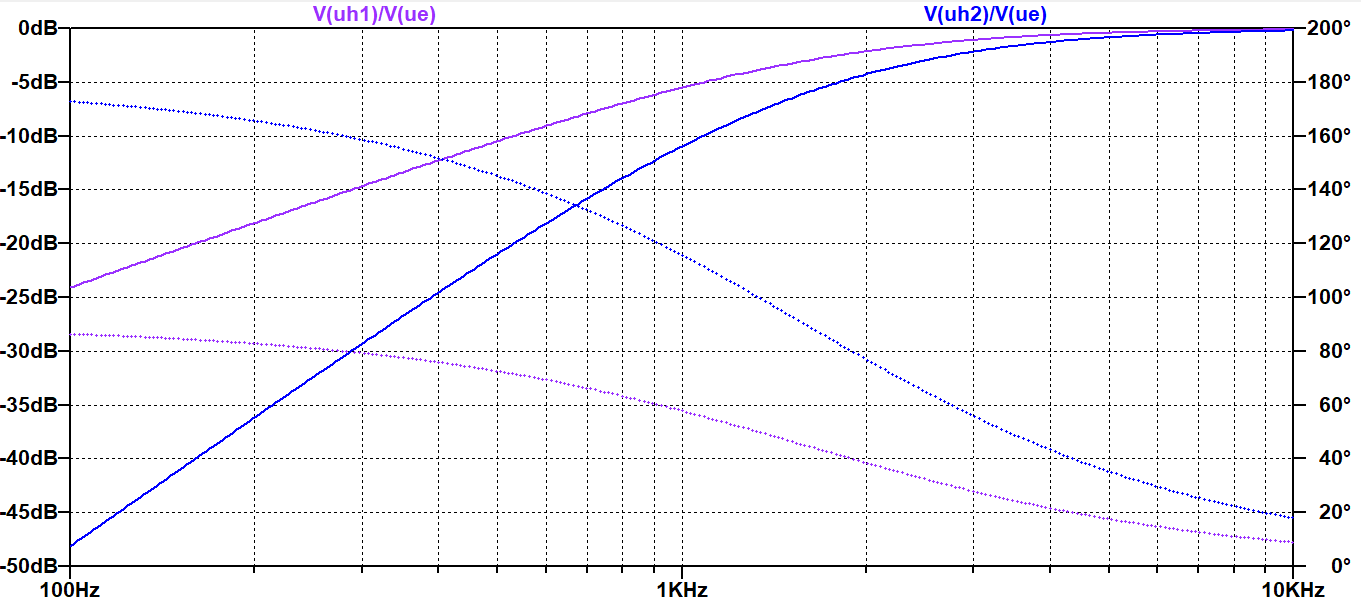
\includegraphics[width=16cm]{./pictures/Hochpass_Bode}
    \caption{Bodediagram des Hochpasses}
    \label{fig:HochpassBode}
\end{figure}

Die blaue Kurve stellt den gesamten Hochpass dar, die violette Kurve nur einen einfachen Hochpass. Somit erkennt man anhand der Steigung einen Hochpass der Ordnung 2.

\newpage
\begin{figure}[htb]
    \includegraphics[width=14cm]{./pictures/Tiefpass}
    \caption{Aufbau des Tiefpasses}
    \label{fig:Tiefpass}
\end{figure}

\begin{figure}[htb]
    \includegraphics[width=14cm]{./pictures/Aufbau/Tiefpass}
    \caption{Praktischer Aufbau des Tiefpasses (links)}
    \label{fig:TiefpassPraktisch}
\end{figure}

In der Aufgabenstellung wird zudem ein Tiefpass der Ordnung zwei gefordert. Diese Anforderung realisieren wir mittels zwei typischer RC-Tiefpässe. Diese sind über einen Spannungsfolger gekoppelt. Der gesamte Tiefpass ist mit einem weiteren Spannungsfolger vom weiteren Verlauf der Schaltung sicher in Hinsicht auf Rückkopplungen und unzulässiger Ströme abgetrennt.

Wir wählen für unsere Kondensatoren und Widerstände die analogen Werte zum Hochpass, da wir dieselbe Grenzfrequenz anstreben und die Frequenzformel des Hochpasses analog für den Tiefpass gilt. Somit erhalten wir auch hier eine Grenzfrequenz von $1591.6Hz$.

\newpage
Die Übertragungsfunktion ergibt sich gleichermaßen aus der Spannungsteilerregel und dem Verhältnis $U_{t2}$ zu $U_{e}$:
\gleichung{
\begin{split}
&\frac{U_a}{U_e} = \frac{C}{((R+C)||C)+R}
\\
&R+C = R+\frac{1}{j \omega C} = R-j \frac{1}{\omega C}
\\
&(R+C)||C) = \frac{(-j \frac{1}{\omega C})(R-j \frac{1}{\omega C})}{(R-j \frac{1}{\omega C})-j \frac{1}{\omega C}}
\end{split}
}{}
\gleichung{
\begin{split}
\frac{C}{(R+C)||C)} &= \frac{-j \frac{1}{\omega C}}{\frac{(-j \frac{1}{\omega C})(R-j \frac{1}{\omega C})}{(R-j \frac{1}{\omega C})-j \frac{1}{\omega C}}+R}
\\
&= \frac{-j \frac{1}{\omega C}}{\frac{-j \frac{R}{\omega C} - \frac{1}{(\omega C)^2}}{R-j \frac{2}{\omega C}}+R}
\\
&= \frac{\omega CR-j\frac{2\omega C}{\omega C}}{1-jR\omega C+(\omega CR)^2-j\frac{2R(\omega C)^2}{\omega C}}
\\
&= \frac{\omega CR-2j}{1+(\omega CR)^2-3jR\omega C}
\end{split}
}{}
\gleichung{
U_{a}(f) = \frac{\omega CR-2j}{1+(\omega CR)^2-3jR\omega C} * U_{e}(f)
}{}

\newpage
\begin{figure}[htb]
    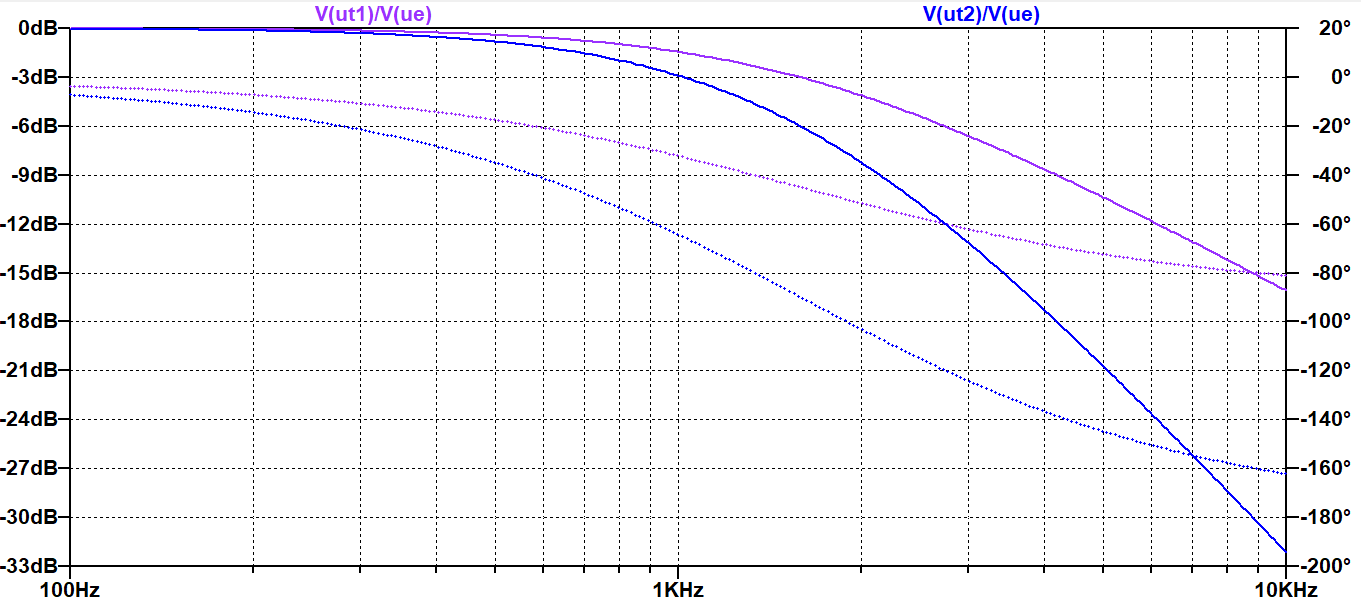
\includegraphics[width=16cm]{./pictures/Tiefpass_Bode}
    \caption{Bodediagram des Tiefpasses}
    \label{fig:TiefpassBode}
\end{figure}

Die blaue Kurve stellt den gesamten Tiefpass dar, die violette Kurve nur einen einfachen Tiefpass. Somit erkennt man anhand der Steigung einen Tiefpass der Ordnung 2.

\subsubsection{Ergebnisse}

\begin{figure}[htb]
    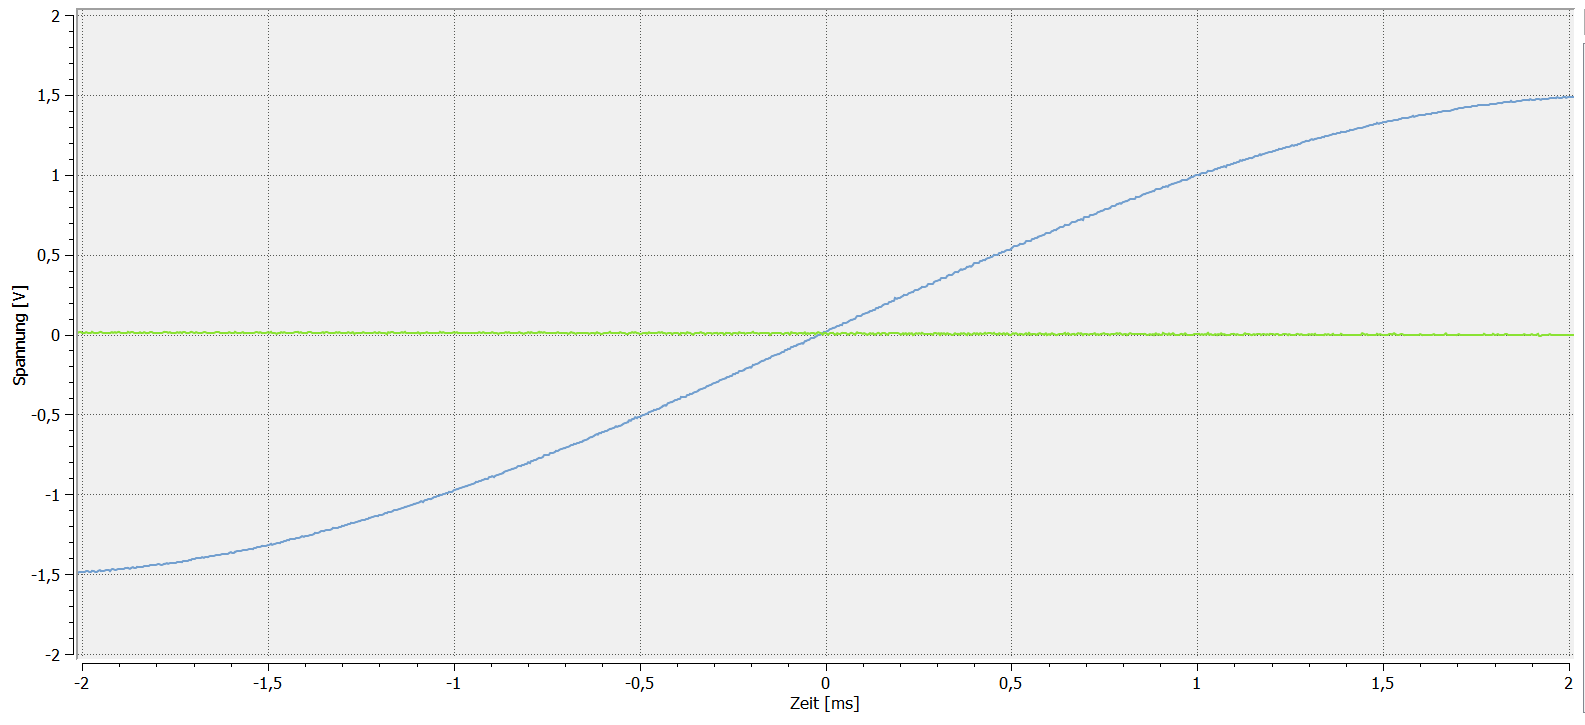
\includegraphics[width=16cm]{./pictures/Messungen/Hochpass_114}
    \caption{Praktische Messung des Hochpasses bei $f=114Hz$}
    \label{fig:Hochpass_114}
\end{figure}

\newpage
\begin{figure}[htb]
    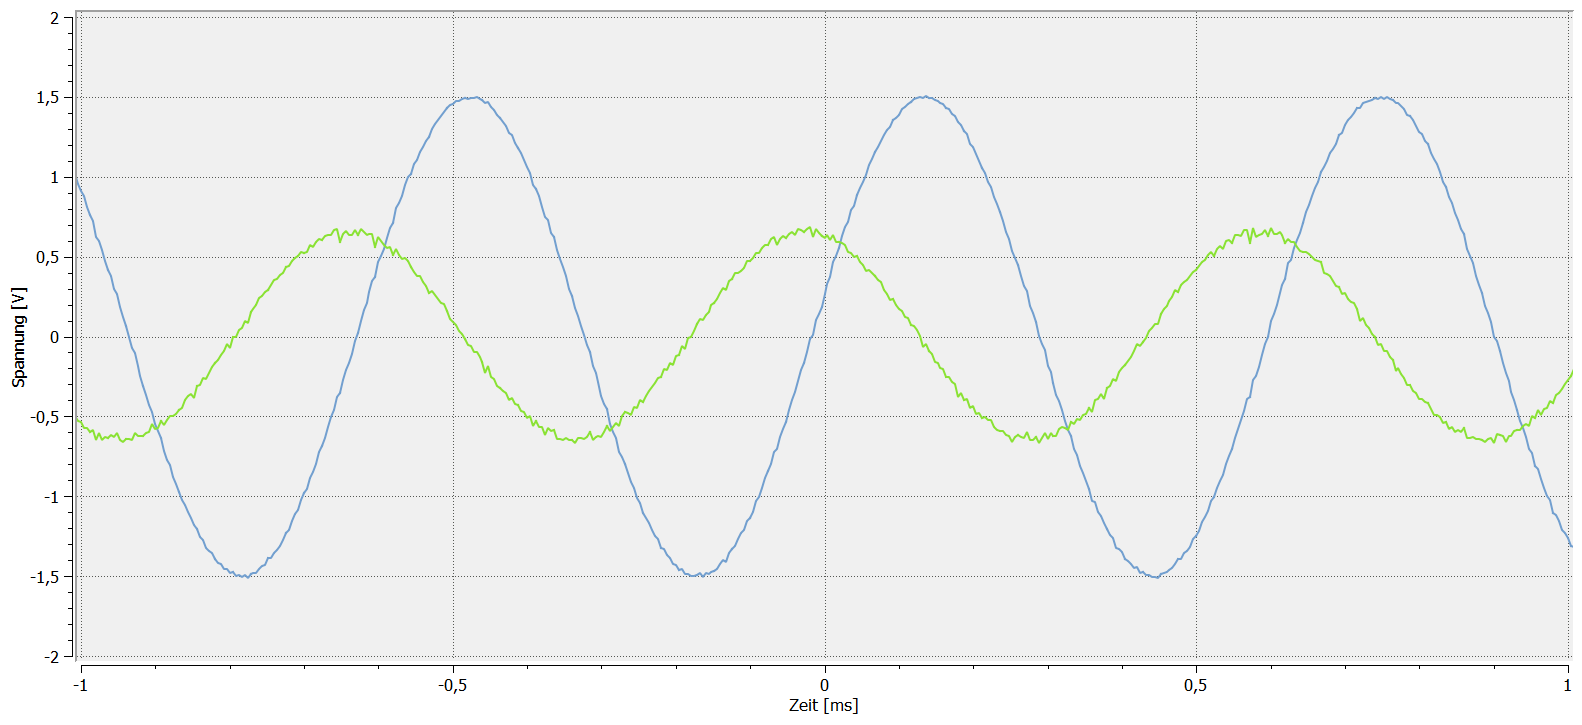
\includegraphics[width=13cm]{./pictures/Messungen/Hochpass_1,63k}
    \caption{Praktische Messung des Hochpasses bei $f=1.63kHz$}
    \label{fig:Hochpass_1,63k}
\end{figure}

\begin{figure}[htb]
    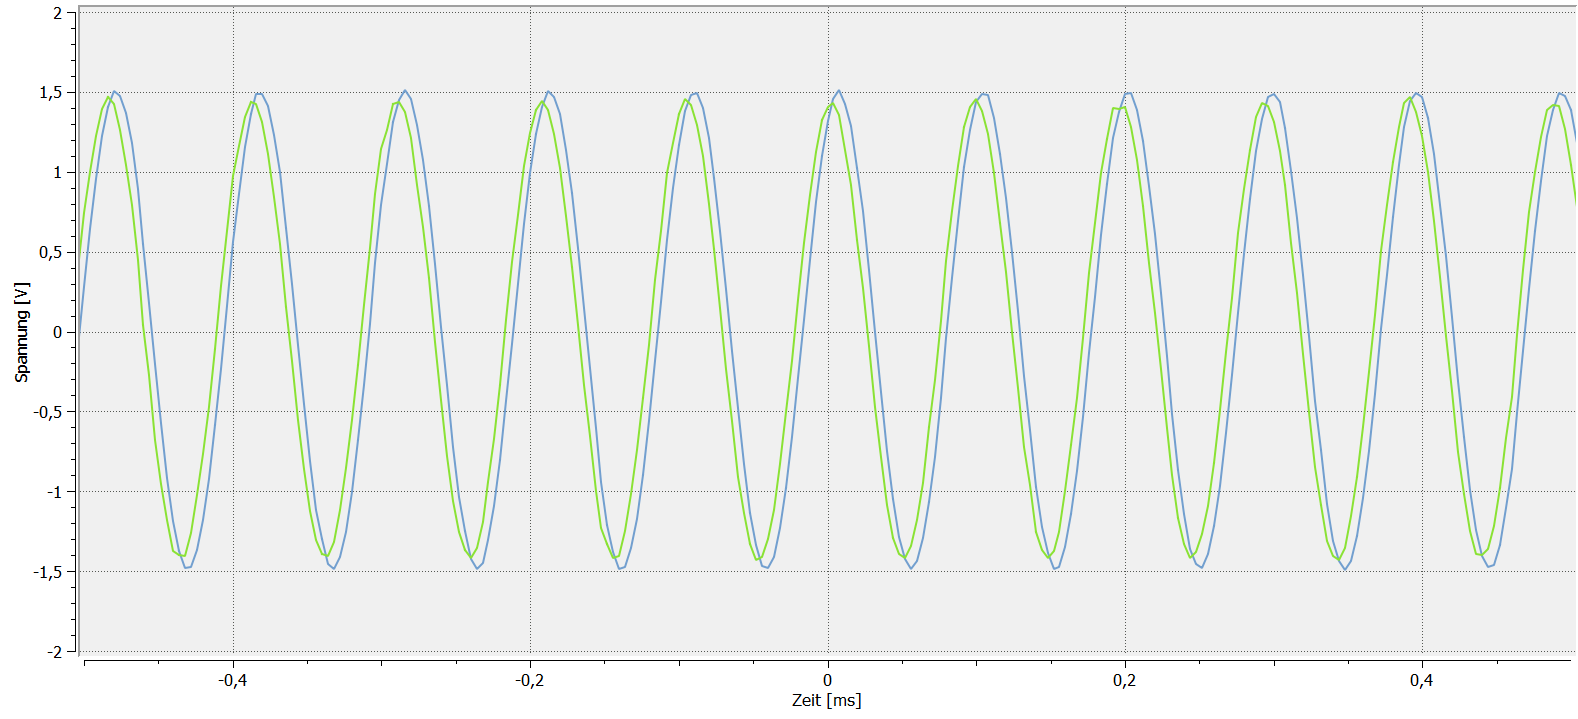
\includegraphics[width=13cm]{./pictures/Messungen/Hochpass_10k}
    \caption{Praktische Messung des Hochpasses bei $f=10kHz$}
    \label{fig:Hochpass_10k}
\end{figure}

~\\
Bei den Bildern des Hochpasses stellt die blaue Kurve unser Eingangssignal und die grüne Kurve unser Ausgangssignal dar.
\\
\\
Bei $f=114Hz$ (Abbildung \ref{fig:Hochpass_114}) wird die Eingangsspannung maximal gedämpft. Dies zeigt sich durch eine quasi konstante Ausgangsspannung bei 0V. Dieses Verhalten erwarten wir von einem Hochpass.
\\
\\
Bei $f=1.63kHz$ (Abbildung \ref{fig:Hochpass_1,63k}) (nah unserer Grenzfrequenz) wird die Eingangsspannung ca. halb gedämpft. Dies kann man an den Amplituden der sinusförmigen Spannungsbilder ablesen und ergibt sich aus den -3dB Verstärkung bei der Grenzfrequenz.
\\
\\
Bei $f=10kHz$ (Abbildung \ref{fig:Hochpass_10k}) wird die Eingangsspannung infinitesimal klein gedämpft. Hierbei überlappen sich Ein- und Ausgangsspannung. Wir erwarten dieses Verhalten bei einem Hochpass.

\newpage
\begin{figure}[htb]
    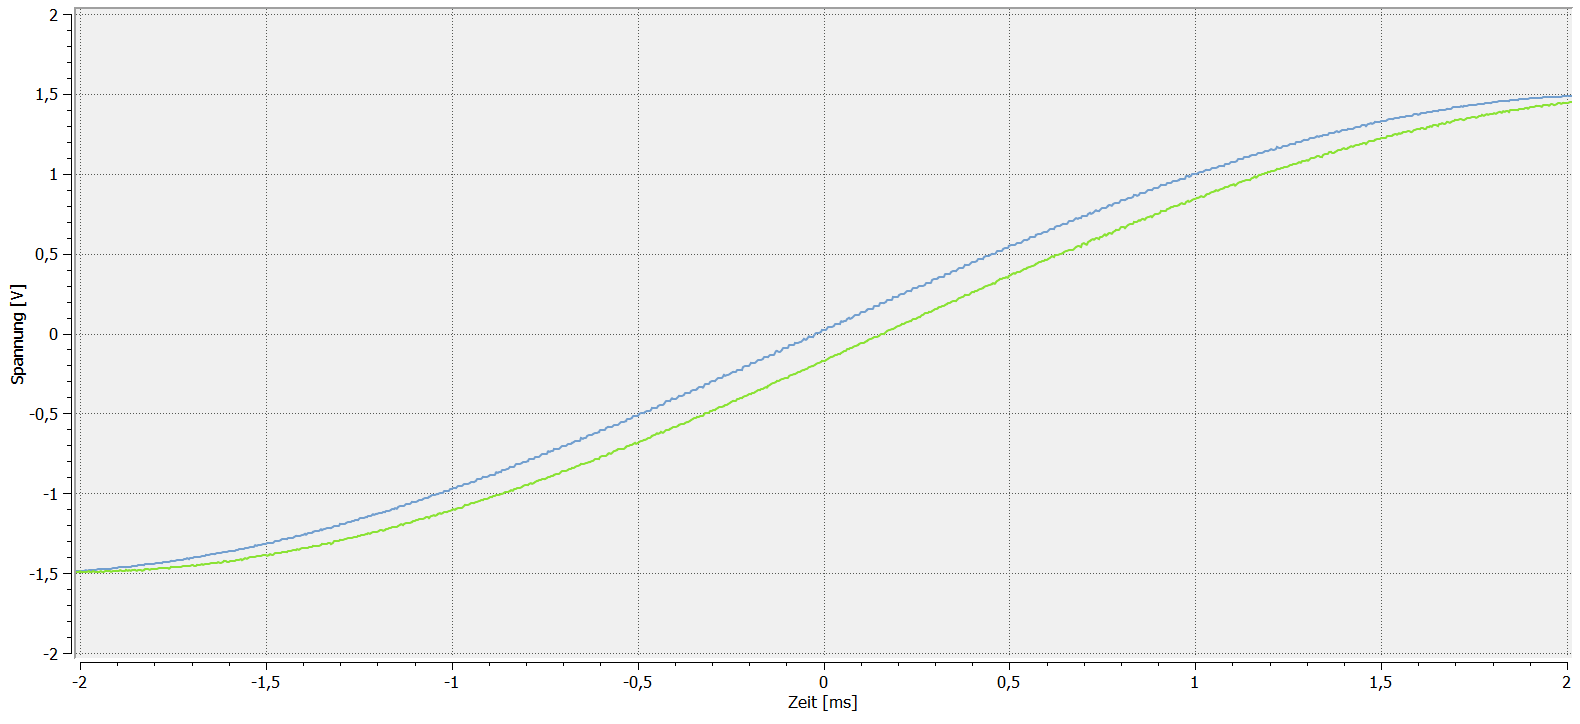
\includegraphics[width=16cm]{./pictures/Messungen/Tiefpass_114}
    \caption{Praktische Messung des Tiefpasses bei $f=114Hz$}
    \label{fig:Tiefpass_114}
\end{figure}

\begin{figure}[htb]
    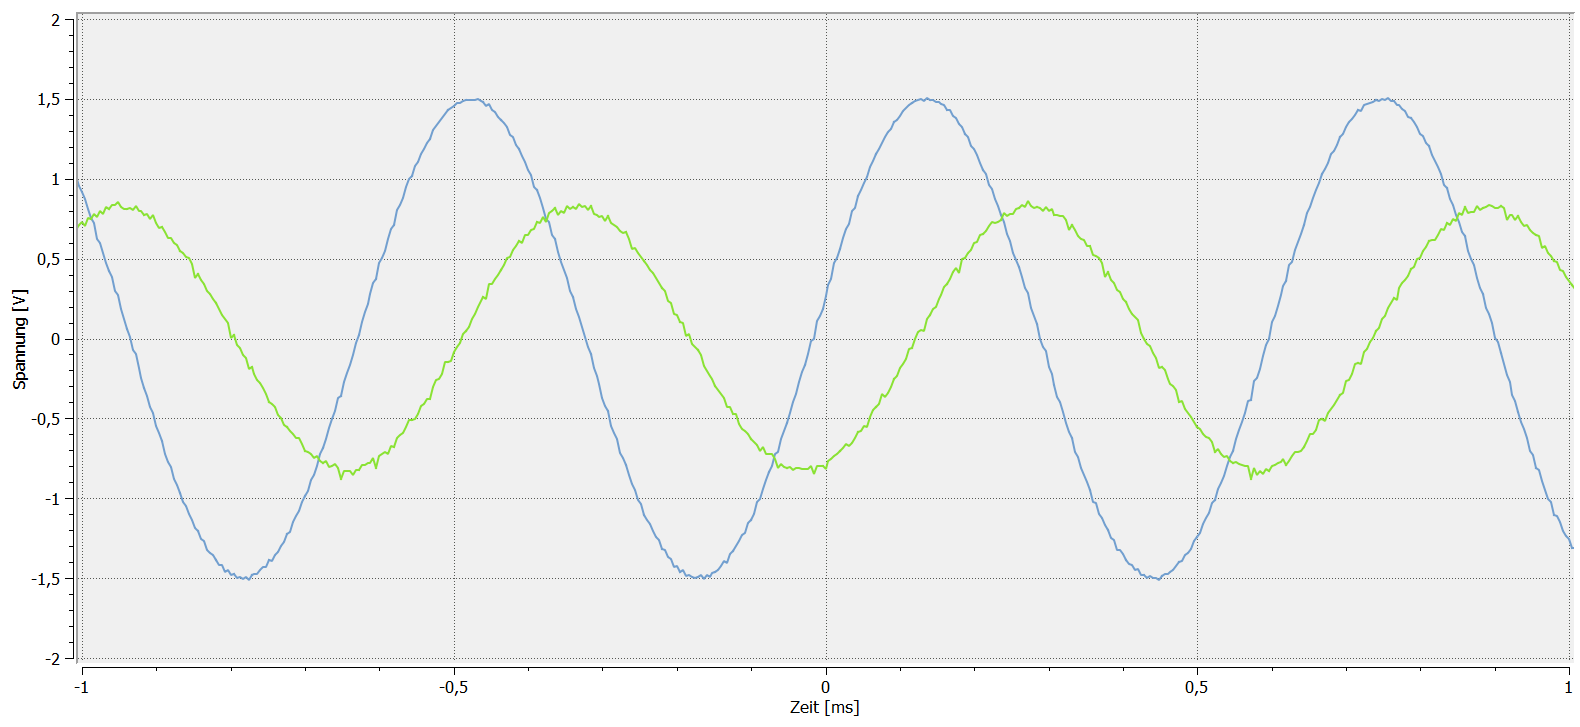
\includegraphics[width=16cm]{./pictures/Messungen/Tiefpass_1,63k}
    \caption{Praktische Messung des Tiefpasses bei $f=1.63kH$}
    \label{fig:Tiefpass_1,63k}
\end{figure}

\newpage
\begin{figure}[htb]
    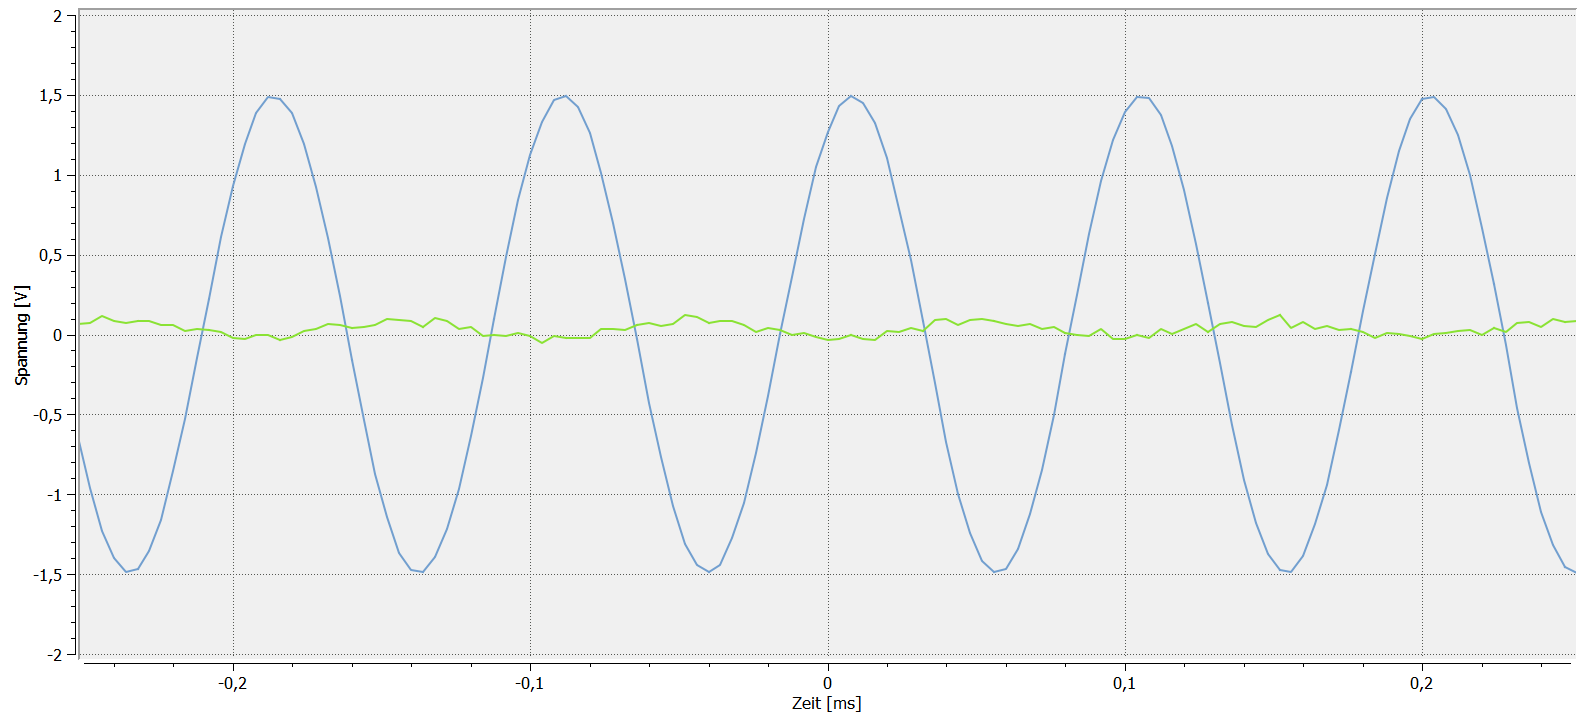
\includegraphics[width=13cm]{./pictures/Messungen/Tiefpass_10k}
    \caption{Praktische Messung des Tiefpasses bei $f=10kHz$}
    \label{fig:Tiefpass_10k}
\end{figure}

Bei den Bildern des Tiefpasses stellt die blaue Kurve unser Eingangssignal und die grüne Kurve unser Ausgangssignal dar.
\\
\\
Bei $f=114Hz$ (Abbildung \ref{fig:Tiefpass_114}) wird die Eingangsspannung infinitesimal klein gedämpft.  Die Amplitude des Ein- und Ausgangssignals ist dabei quasi identisch.
\\
\\
Bei $f=1.63kHz$ (Abbildung \ref{fig:Tiefpass_1,63k}) (nah unserer Grenzfrequenz) wird die Eingangsspannung ca. halb gedämpft. Dies kann man an den Amplituden der sinusförmigen Spannungsbilder ablesen und ergibt sich aus den -3dB Verstärkung bei der Grenzfrequenz. Dieses Spannungsbild ist dem des Hochpasses bei dieser Frequenz fast gleich.
\\
\\
Bei $f=10kHz$ (Abbildung \ref{fig:Tiefpass_10k}) wird die Eingangsspannung maximal gedämpft. Dies zeigt sich durch eine quasi konstante Ausgangsspannung bei 0V. Dieses Verhalten erwarten wir von einem Tiefpass.

\begin{figure}[htb]
    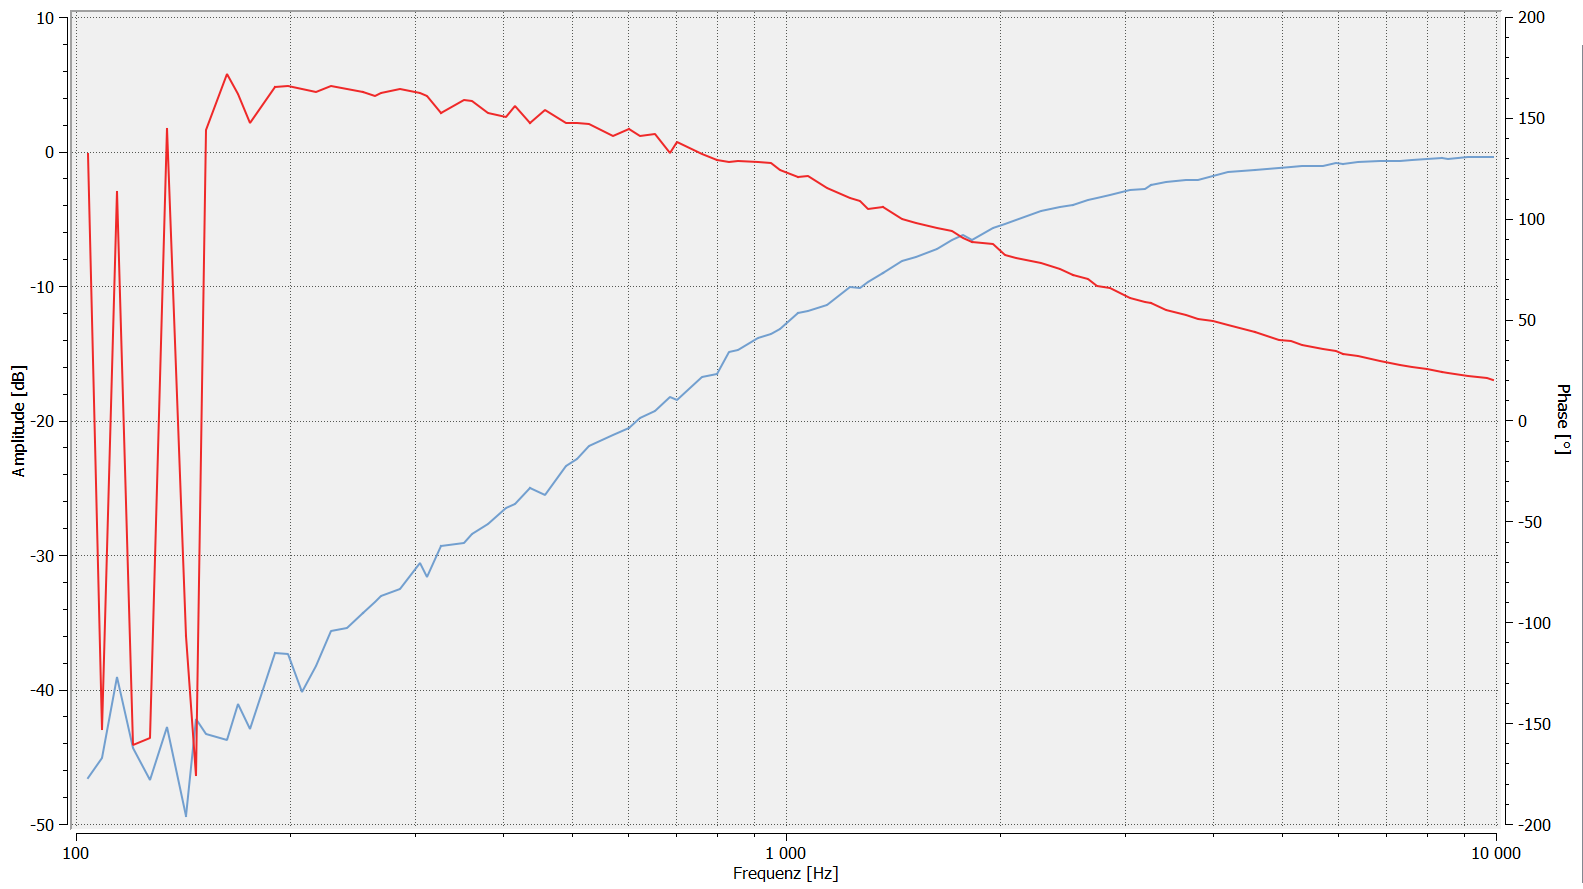
\includegraphics[width=13cm]{./pictures/Messungen/Hochpass_Bode_Test}
    \caption{Gemessenes Bode-Diagramm des Hochpasses}
    \label{fig:Hochpass_Bode_Test}
\end{figure}

\newpage

\begin{figure}[htb]
    \includegraphics[width=14cm]{./pictures/Messungen/tiefpass_Bode_Test}
    \caption{Gemessenes Bode-Diagramm des Tiefpasses}
    \label{fig:Tiefpass_Bode_Test}
\end{figure}

\subsubsection{Diskussion}

Unsere beiden Filterschaltungen funktionieren in der Praxis simultan zum simulierten Verhalten. Dabei treten zwar kleine Messungenauigkeiten auf, jedoch verhalten sich Phasen- und Amplitudengänge der Ausgangsspannungen wie erwartet für die konstruierten Filter. Der Hochpass filtert tiefe Frequenzen der Ausgangsspannung, der Tiefpass filtert hohe Frequenzen. 
\\
\\
Die gemessenen Bode-Diagramme des Hoch- und Tiefpasses stimmen mit den simulierten Diagrammen überein. Dabei treten beim Hochpass Messfehler bei sehr kleinen Frequenzen auf, aber der allgemeine Kurvenverlauf ist gleich. Die Messfehler kommen durch das Programm LenLab oder durch äußere Einflüsse zustande.

\newpage
\subsection{Addierschaltung}

\subsubsection{Materialien \& Methoden}

\begin{figure}[htb]
    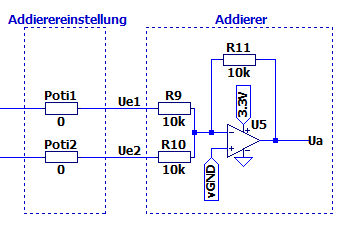
\includegraphics[width=14cm]{./pictures/Addierer}
    \caption{Addiererschaltung des Hoch- und Tiefpasses}
    \label{fig:Addierer}
\end{figure}

\begin{figure}[htb]
    \includegraphics[width=14cm]{./pictures/Aufbau/Gesamtschaltung}
    \caption{Praktischer Aufbau der Gesamtschaltung}
    \label{fig:GesamtschaltungPraktisch}
\end{figure}

\newpage
\begin{figure}[htb]
    \includegraphics[width=14cm]{./pictures/Aufbau/Ueberlagerung}
    \caption{Praktischer Aufbau der Überlagerungsschaltung}
    \label{fig:Überlagerung}
\end{figure}

\begin{figure}[htb]
    \includegraphics[width=16cm]{./pictures/Gesamtschaltung}
    \caption{Ausgangsspannung des Addierers}
    \label{fig:AddiererAusgangsspannung}
\end{figure}

Die ermittelte Kurve zeigt, dass einer der Filter eine negative Spannung erzeugt. Nach weiteren Simulationen mit Spice wurde festgestellt, dass der Tiefpass negative Spannungen erzeugt. Aufgrund dessen muss das Ausgangssignal des Tiefpasses invertiert werden, da sonst die Ausgangssignale nicht addiert, sonst subtrahiert werden.

\newpage

\begin{figure}[htb]
    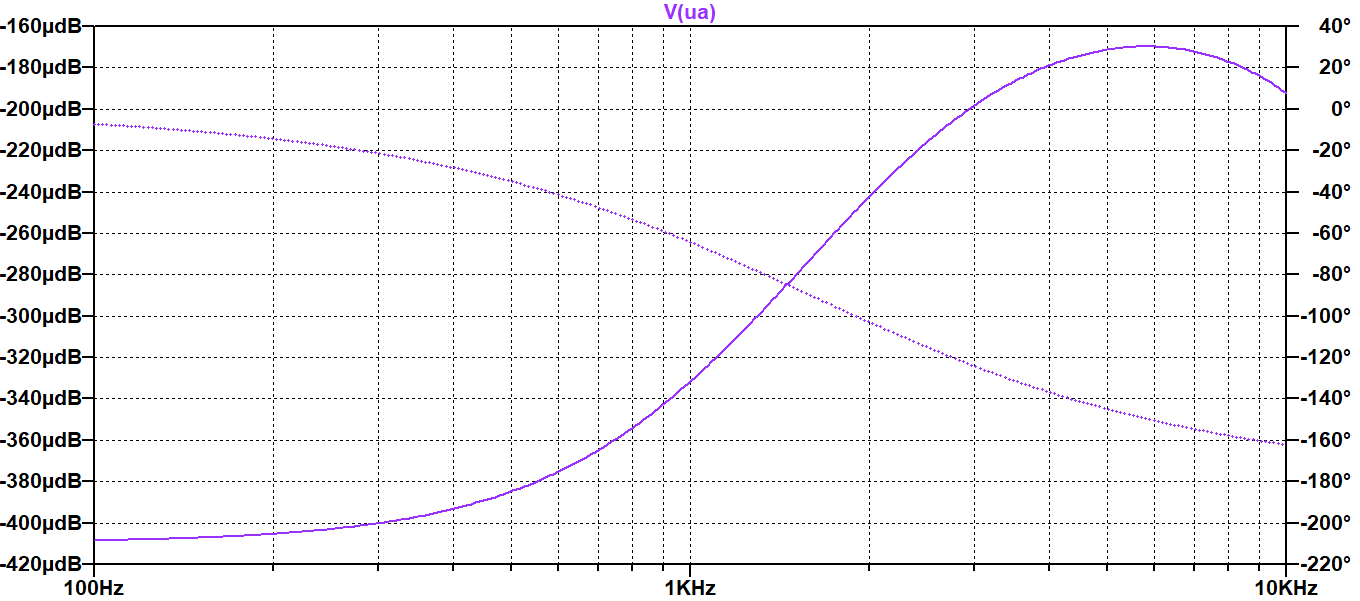
\includegraphics[width=16cm]{./pictures/Gesamtschaltung_Invertiert}
    \caption{Ausgangsspannung des Addierers mit invertiertem Tiefpass mit $R_1 = R_2 = 0$}
    \label{fig:AddiererAusgangsspannungInvertiert}
\end{figure}

Wir beobachten nun eine maximale Dämpfung des Signals bei 100Hz und Maximum bei ca. 6000Hz. Die Funktion verläuft nun stetig ohne abrupte Änderung.
\\
\\
Einen solchen Filter bezeichnet man als 2-Band-Equalizer, da dieser aus einem kombinierten Hoch- und Tiefpass besteht und die jeweiligen Ausgangssignale des Hoch- und Tiefpasses einstellbar kombiniert werden können.

\begin{figure}[htb]
    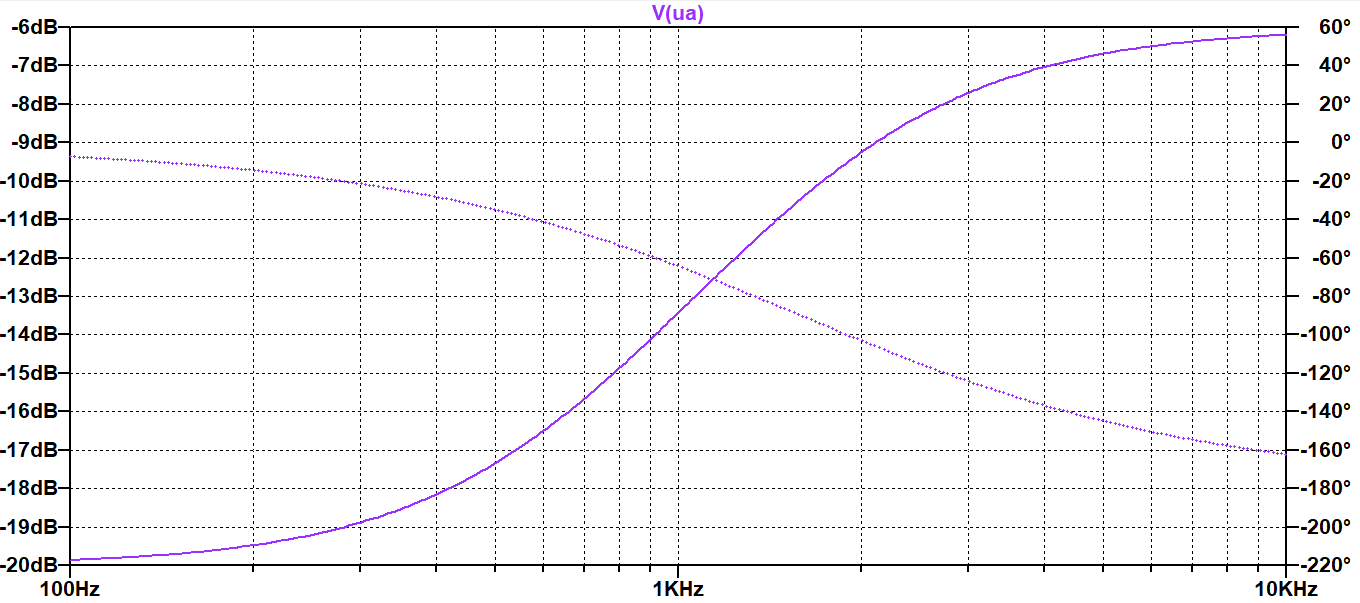
\includegraphics[width=16cm]{./pictures/Gesamtschaltung_Invertiert_10_90}
    \caption{Ausgangsspannung des Addierers mit invertiertem Tiefpass mit $R_1 = 10k\Omega$ und $R_2 = 90k\Omega$}
    \label{fig:AddiererAusgangsspannungInvertiert}
\end{figure}

\newpage

\begin{figure}[htb]
    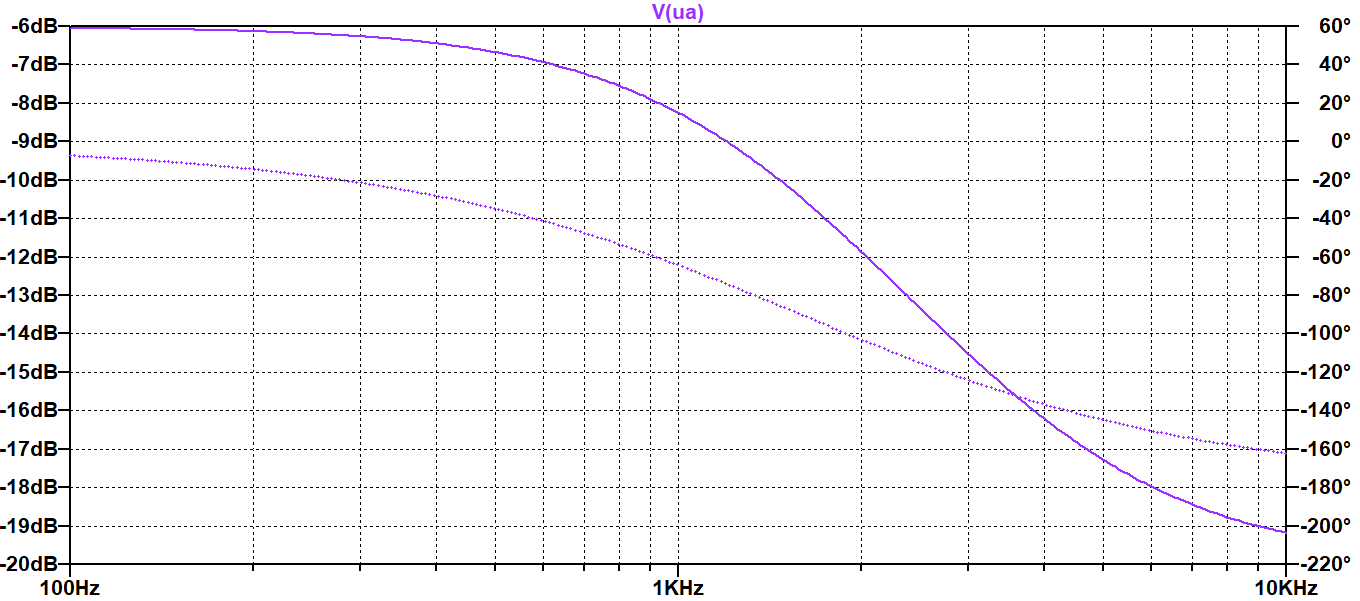
\includegraphics[width=16cm]{./pictures/Gesamtschaltung_Invertiert_90_10}
    \caption{Ausgangsspannung des Addierers mit invertiertem Tiefpass mit $R_1 = 90k\Omega$ und $R_2 = 10k\Omega$}
    \label{fig:AddiererAusgangsspannungInvertiert}
\end{figure}

Durch die Einstellungen an den Potentiometern lässt sich einstellen, welche Frequenzbereiche gedämpft werden sollen.

\subsubsection{Ergebnisse}

\begin{figure}[htb]
    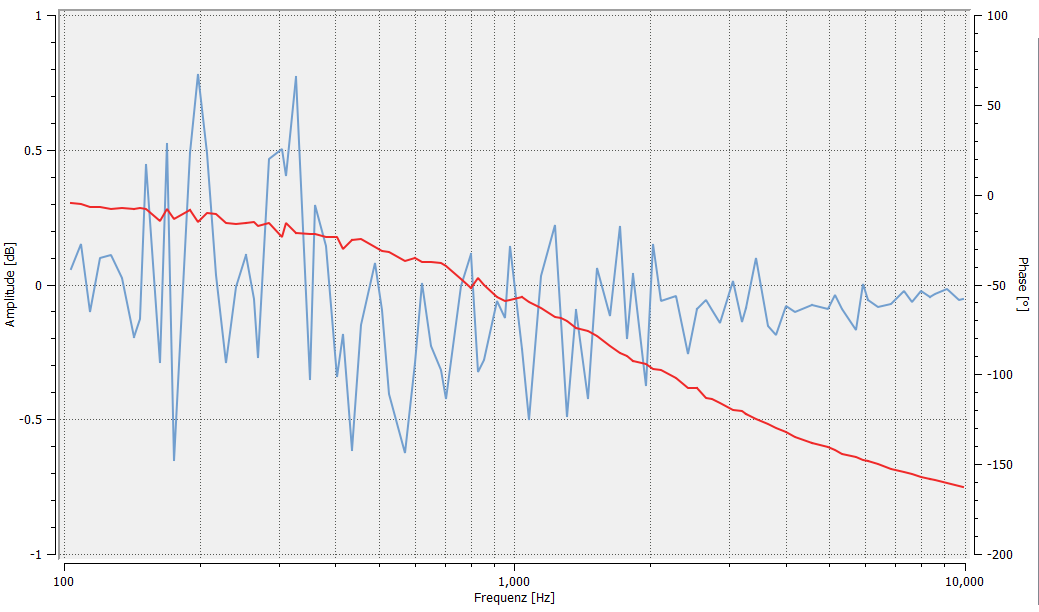
\includegraphics[width=16cm]{./pictures/Messungen/Gesamtschaltung_Test_0_0}
    \caption{Gemessene Ausgangsspannung mit $R_1 = 0\Omega$ und $R_2 = 0\Omega$}
    \label{fig:Gesamtschaltung_Test_0_0}
\end{figure}

\newpage

\begin{figure}[htb]
    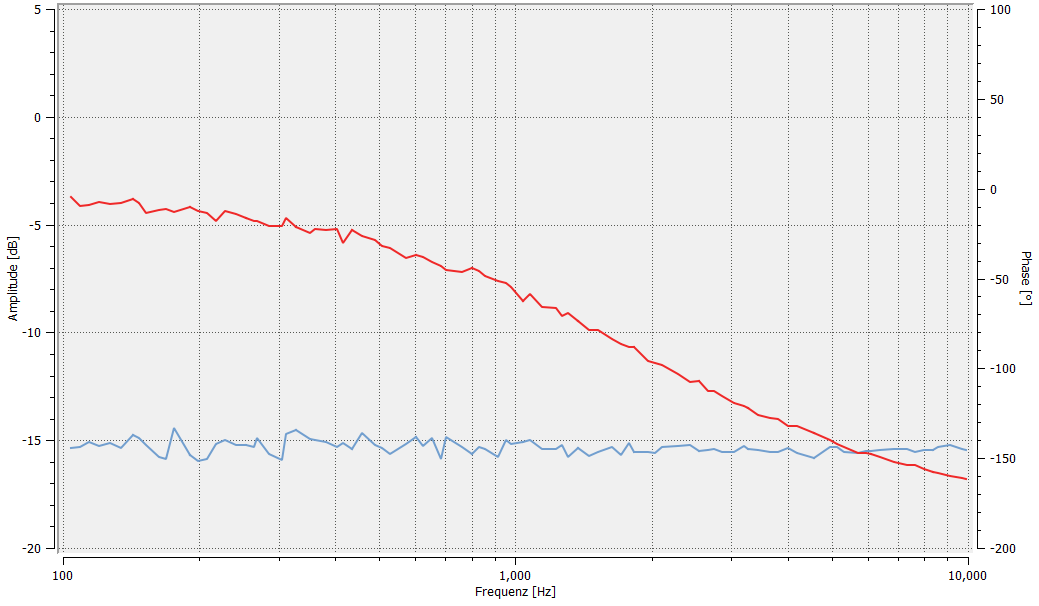
\includegraphics[width=16cm]{./pictures/Messungen/Gesamtschaltung_Test_50_50}
    \caption{Gemessene Ausgangsspannung mit $R_1 = 50k\Omega$ und $R_2 = 50k\Omega$}
    \label{fig:Gesamtschaltung_Test_50_50}
\end{figure}

\begin{figure}[htb]
    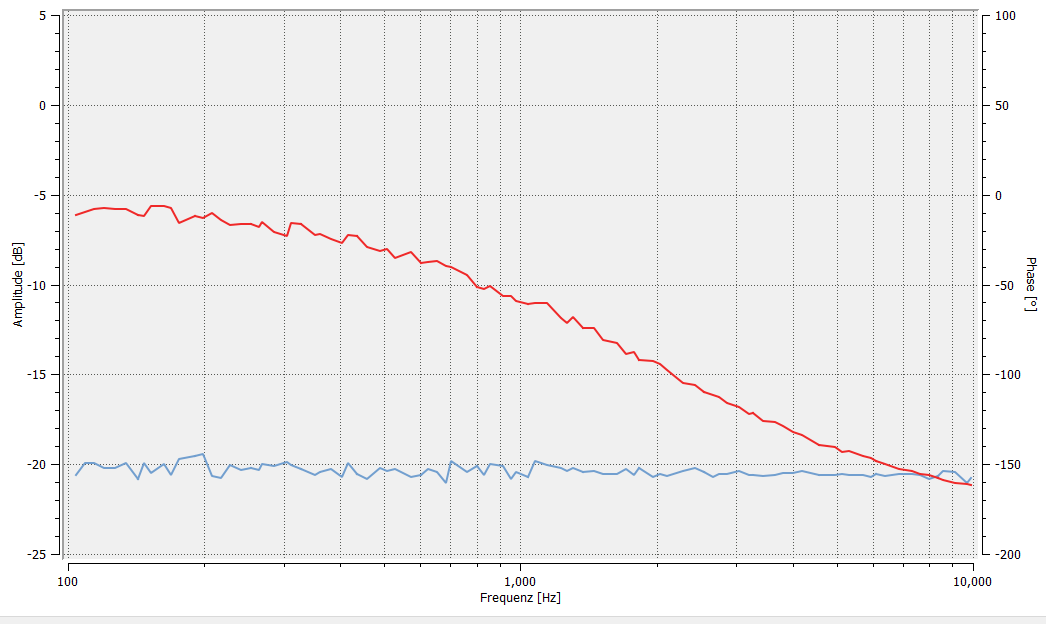
\includegraphics[width=16cm]{./pictures/Messungen/Gesamtschaltung_Test_100_100}
    \caption{Gemessene Ausgangsspannung mit $R_1 = 100k\Omega$ und $R_2 = 100k\Omega$}
    \label{fig:Gesamtschaltung_Test_100_100}
\end{figure}

\newpage

\begin{figure}[htb]
    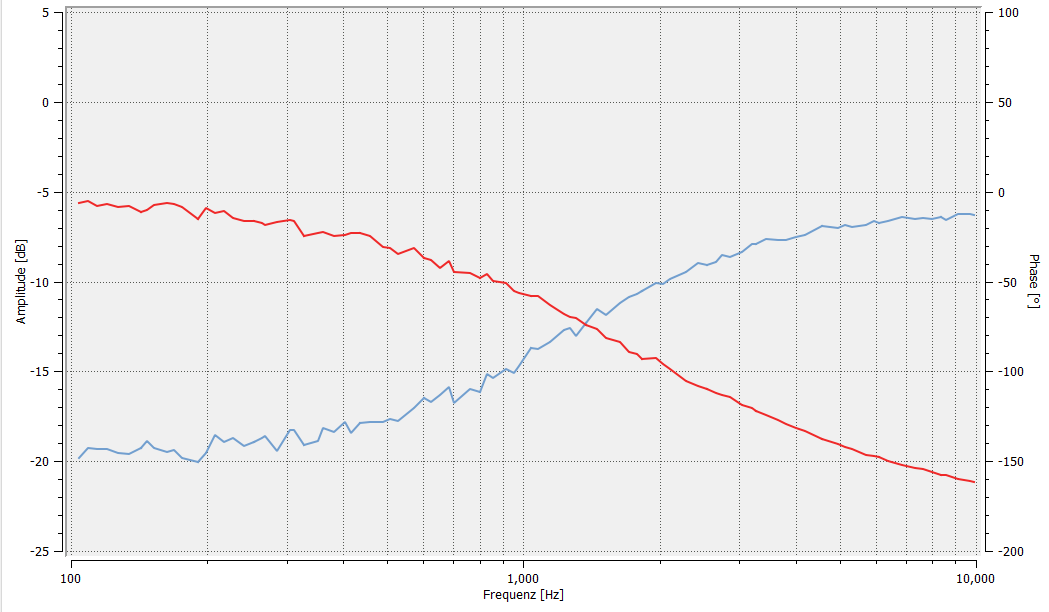
\includegraphics[width=16cm]{./pictures/Messungen/Gesamtschaltung_Test_10_90}
    \caption{Gemessene Ausgangsspannung mit $R_1 = 10k\Omega$ und $R_2 = 90k\Omega$}
    \label{fig:Gesamtschaltung_Test_10_90}
\end{figure}

\begin{figure}[htb]
    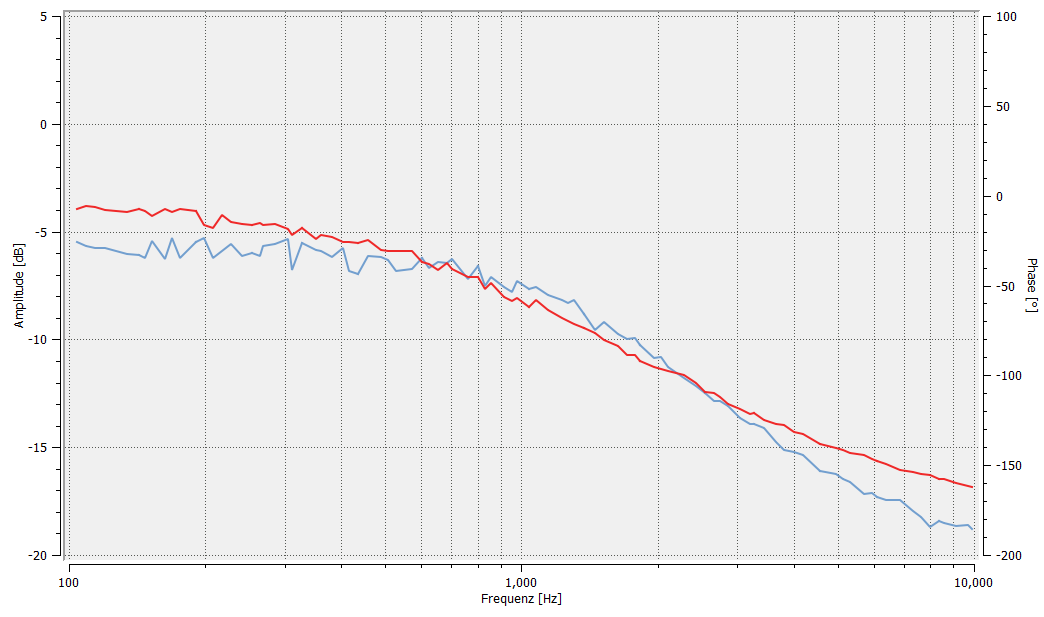
\includegraphics[width=16cm]{./pictures/Messungen/Gesamtschaltung_Test_90_10}
    \caption{Gemessene Ausgangsspannung mit $R_1 = 90k\Omega$ und $R_2 = 10k\Omega$}
    \label{fig:Gesamtschaltung_Test_90_10}
\end{figure}

Die blaue Kurve stellt den Amplitudenverlauf der Ausgangsspannung dar, die rote Kurve den Phasenverlauf.

\newpage

\begin{figure}[htb]
    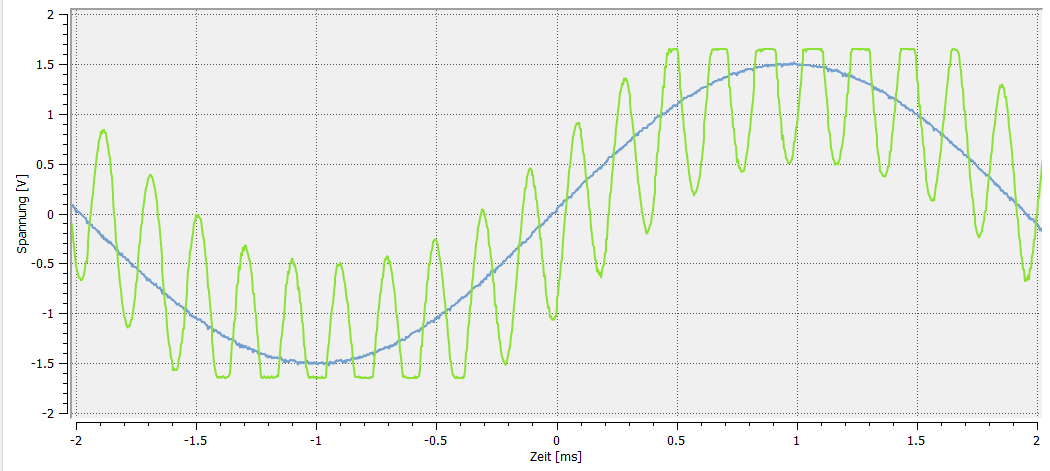
\includegraphics[width=16cm]{./pictures/Messungen/Ueberlagerung_100_0}
    \caption{Gemessene Ausgangsspannung bei $f_{1} = 254Hz$ und $f_{2} = 5080Hz$ mit $R_1 = 100k\Omega$ und $R_2 = 0\Omega$}
    \label{fig:Überlagerung_100_0}
\end{figure}

\begin{figure}[htb]
    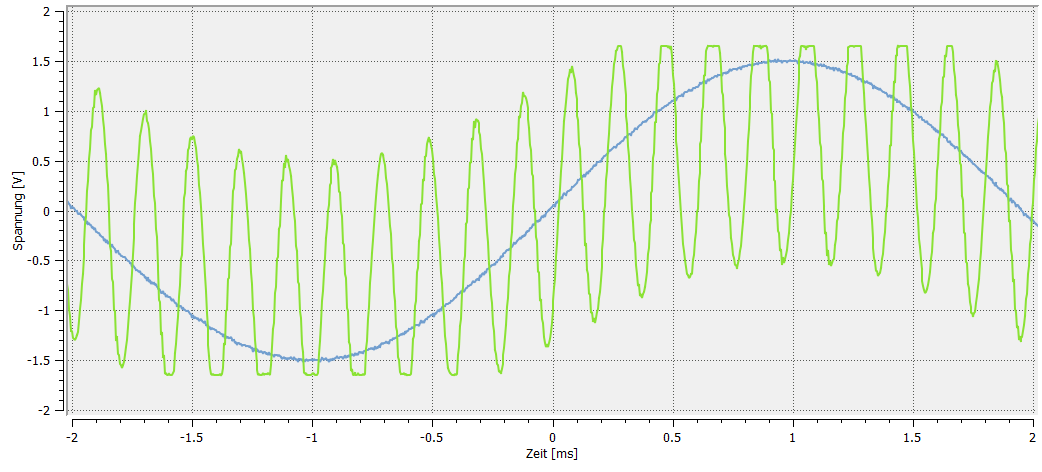
\includegraphics[width=16cm]{./pictures/Messungen/Ueberlagerung_0_100}
    \caption{Gemessene Ausgangsspannung bei $f_{1} = 254Hz$ und $f_{2} = 5080Hz$ mit $R_1 = 0\Omega$ und $R_2 = 100k\Omega$}
    \label{fig:Überlagerung_0_100}
\end{figure}

\subsubsection{Diskussion}

Unsere gemessenen Bildern mit unterschiedlichen Poti-Einstellungen ähneln den simulierten Werten stark. Bei Messungen mit $R_1 = 0\Omega$ und $R_2 = 0\Omega$ treten große Messfehler bezüglich der Spannung auf, die Phase ist deckungsgleich zu der der Simulation.
\\
\\
Bei gleichen Werten der beiden Potis lässt sich eine waagerechte Übertragungsfunktion erkennen. Dieses Verhalten haben wir erwartet, da die Signale des Hoch- und Tiefpasses äquivalent verrechnet werden.
\\
\\
Die Poti-Einstellungen bei $R_1 = 10k\Omega$ und $R_2 = 90k\Omega$ und bei $R_1 = 90k\Omega$ und $R_2 = 10k\Omega$ ergeben deckungsgleiche Verläufe der simulierten und gemessenen Ergebnissen. Im einen Fall werden tiefe Frequenzen gedämpft, im anderen werden hohe Frequenzen äquivalent gedämpft, wie wir es von unserem Equalizer erwarten.
\\
\\
\\
In den beiden Darstellungen stellt der blaue Graph die Eingansspannung mit 254Hz dar, die auf den Eingang des Equalizers gegeben wird und die grüne Kurve stellt das gemessene Ausgangssignal dar. Die beiden Eingangssignale werden mit einem zweiten Spannungsteiler überlagert, der dem Spannungsteiler der virtuellen Masse baugleich ist. 
\\
\\
Bei hohen Hochpasswerten ($R_{1} = 100k\Omega$ und $R_{2} = 0\Omega$) wird der tiefe Frequenzanteil gedämpft. Der hohe Frequenzanteil bleibt erhalten. Dies erkennt man an der Äquivalenz der Amplituden des Ein- und Ausgangssignals und der Schwingung um 0V des Ausganssignals.
\\
Bei hohen Tiefpasswerten ($R_{1} = 0\Omega$ und $R_{2} = 100k\Omega$) lässt sich eine starke Dämpfung der hohen Frequenzanteile des Ausgangssignals im Vergleich zum Eingangssignal erkennen. Die niedrigen Frequenzanteile werden jedoch nicht gedämpft. Die Ausgansspannung verläuft Phasengleich zur Eingangsspannung.
\\
\\
Im Praxistest hat sich die Schaltung bewährt. Ein eingespeistes Musiksignal konnte mittels der Potis beeinflusst werden und somit hohe und Tiefe Tonfrequenzen reguliert werden. Auffällig war die schlechte Qualität (Rauschen) des Ausgangssignals. Wir schreiben dieses Rauschen der mangelnden Abschirmung und den schlechten Kontakten zwischen den einzelnen Bauteilen zu.

\newpage
\begin{sidewaysfigure}[htb]
    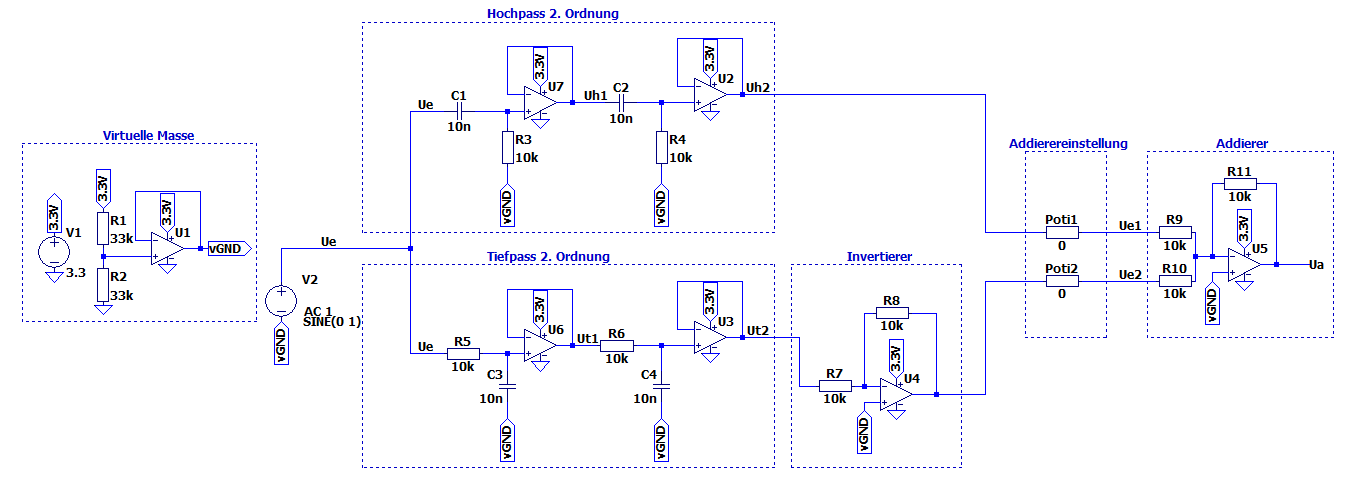
\includegraphics[width=22cm]{./pictures/Schaltung}
    \caption{Gesamtschaltung des Filters}
    \label{fig:Gesamtschaltung}
\end{sidewaysfigure}

\clearpage % neue Seite beginnen
\section{Literaturverzeichnis}

\begin{thebibliography}{99}
\bibitem{tkotz}Klaus Tkotz. {\itshape Fachkunde Elektrotechnik}. Verlag Europa-Lehrmittel GmbH \& Co., Ostfildern, 28. Auflage, 2012.
\bibitem{lutz}Lutz v. Wangenheim. {\itshape Aktive Filter und Oszillatoren}. Springer Verlag Berlin-Heidelberg, 2008
\bibitem{kendall}Kendall Su. {\itshape ANALOG FILTERS, SECOND EDITION}. Kluwer Academic Publishers group, 2008
\bibitem{tietze}Ulrich Tietze, Christoph Schenk, Eberhard Gamm. {\itshape Halbleiter Schaltungstechnik}. Springer Verlag Berlin-Heidelberg, 14. Auflage, 2016
\end{thebibliography}

\end{document}

